\documentclass[aspectratio=169]{beamer}
\usetheme{Madrid}
\usepackage[utf8]{inputenc}
\usepackage[T1]{fontenc}
\usepackage{tikz}
\usepackage{amssymb}
\usepackage{graphicx}
\setbeamertemplate{navigation symbols}{}
\setbeamercolor{title}{fg=white,bg=violet!70!purple}
\setbeamercolor{frametitle}{fg=white,bg=violet!70!purple}
\setbeamercolor{block title}{bg=violet!70!purple!20,fg=black}
\setbeamercolor{block body}{bg=violet!70!purple!8,fg=black}
\setbeamercolor{item}{fg=violet!70!purple}
\setbeamercolor{itemize item}{fg=violet!70!purple}
\setbeamertemplate{itemize item}[triangle]

\title{Story Studio 1 — Page Basics}
\subtitle{Headings, paragraphs, links, buttons — the tags every page starts with}
\author{ByteForge --- Grade 7 --- Game Maker}
\date{}

\begin{document}

\begin{frame}
    \titlepage
\end{frame}

\begin{frame}{Today's Plan}
    \begin{itemize}
        \item Front Page
        \item Say More
        \item Chapter One
        \item Read More
        \item Call to Action
        \item[$\bigstar$] BOSS --- Ship the Front Page
    \end{itemize}
\end{frame}

\begin{frame}{A heading is a page's title}
    \large
    \begin{itemize}
        \item One big title, shown once near the top
        \item The ONE thing that tells a reader what this whole page is about. This is what a real webpage's \texttt{<h1>} does.
        \item Worked example: a page with TWO heading blocks reads like a book with two titles on the cover — which one is it actually about? That's why real pages almost always use exactly one.
    \end{itemize}

    \begin{center}
    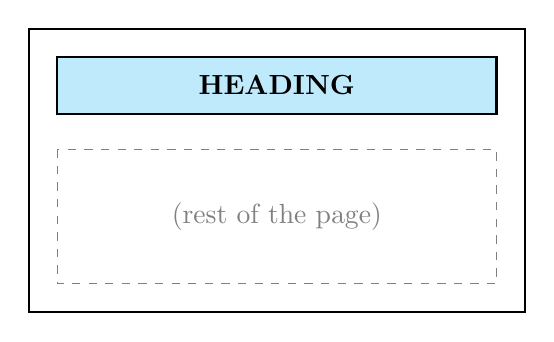
\begin{tikzpicture}[scale=0.9]

        \draw[thick] (0,0) rectangle (7,-4);
        \draw[fill=cyan!25, thick] (0.4,-0.4) rectangle (6.6,-1.2);
        \node at (3.5,-0.8) {\bfseries HEADING};
        \draw[dashed, gray] (0.4,-1.7) rectangle (6.6,-3.6);
        \node[gray] at (3.5,-2.65) {(rest of the page)};
    \end{tikzpicture}
    \end{center}
\end{frame}


\begin{frame}{A paragraph is the body of the page}
    \large
    \begin{itemize}
        \item If the heading is the title, the paragraph is everything you actually want to SAY. Blocks run top to bottom
        \item So does the page.
        \item Worked example: heading "My Story", then paragraph "It was a dark night...". Swap the order and Run — the paragraph now appears ABOVE the heading, because blocks run top to bottom exactly as stacked.
    \end{itemize}
\end{frame}


\begin{frame}{One paragraph per idea}
    \large
    \begin{itemize}
        \item Good writing breaks text into separate paragraphs
        \item One per idea
        \item Rather than one giant block. That's what makes a page skimmable.
    \end{itemize}
\end{frame}


\begin{frame}{A link connects one page to another}
    \large
    \begin{itemize}
        \item Every link needs two things: the text someone clicks, and the address it goes to. Links are what turn separate pages into a connected site.
        \item Worked example: a link block missing its destination is like a signpost with an arrow but no name on it — technically still a signpost, but useless to anyone reading it.
    \end{itemize}
\end{frame}


\begin{frame}{A button invites an action}
    \large
    \begin{itemize}
        \item A link takes you somewhere else; a button triggers something HERE. Right now it does nothing yet
        \item That comes next week.
    \end{itemize}
\end{frame}


\begin{frame}{BOSS — every block, one real page}
    \large
    \begin{itemize}
        \item Heading, paragraphs, link, button is close to the actual shape of a huge number of real websites.
    \end{itemize}
\end{frame}

\begin{frame}{Real-World Examples}
    \large
    \begin{itemize}
        \item Open any news homepage (BBC, a school website) together: point out the ONE big headline, the body paragraphs underneath, a "read more" link, and a "subscribe" button
        \item The exact same four blocks students are about to use. In Minecraft terms: a crafting recipe book page has exactly this shape too
        \item One item name (heading), a description (paragraph), and a "craft" button.
    \end{itemize}
\end{frame}


\begin{frame}{Image}
    \begin{center}
    
\includegraphics[width=0.5\textwidth]{images/html5.png}

    \large The real tag this page-building block stands in for.

    \small HTML5 logo — W3C / Patio, CC BY 3.0, via Wikimedia Commons
    \end{center}
\end{frame}

\begin{frame}{Let Them Discover (1/2)}
    \Large
    Before opening the platform: in pairs, look at 2-3 real websites and list which parts are "heading", "paragraph", "link", or "button". Which pages break the "one heading" rule — and does it make them harder to read?
\end{frame}


\begin{frame}{Let Them Discover (2/2)}
    \Large
    Open Minecraft's recipe book (or a screenshot of one) — find its "heading" (item name), its "paragraph" (ingredients list), and anything that acts like a button. Does every page in the game follow this same shape?
\end{frame}

\begin{frame}{Your Turn}
    \Large
    Open the student map, find \textbf{Story Studio 1 — Page Basics}, and work through it
    hands-on --- everything you just saw, they now do themselves.
\end{frame}

\end{document}
